\section{Testplan}
\subsection{Testfälle}

\subsubsection{Fall 1: Unit Tests}
\begin{enumerate}
\item Systemzustand vor dem Test:\\
	Alle Speicher sind vom System entkoppelt. Je nach Test werden spezielle, virtuelle Speicher angelegt, die auf den jeweiligen Test zugeschnitten sind. Allgemein werden dazu für Abfragen, Änderungs- und Löschaktionen statische Datensätze erstellt, die als Resultate behandelt werden. Für Einfügeaktionen werden leere virtuelle Speicher angenommen.
\item Eingabedaten:\\
	test.php wird aufgerufen. Sonstige Eingaben werden fest im Code der Tests durchgeführt.
\item Erwartete Ereignisse:\\
	Alle Tests liefern ``OK'' zurück
\item Systemzustand nach Test:\\
	Unverändert, wie vor dem Test.
\end{enumerate}

\subsubsection{Fall 2: Installation}
\begin{enumerate}
\item Systemzustand vor dem Test:\\
	1. Durchlauf: Alle Speicher nicht vorhanden, aber die Datenbank. 2. Durchlauf: Speicher sind vorhanden und mit zufälligen Werten gefüllt.
\item Eingabedaten:\\
	install.php wird aufgerufen und die verlangten Daten eingegeben.
\item Erwartete Ereignisse:\\
	Verbindung mit Datenbank wird erstellt, schon vorhandene Speicher gelöscht, Speicher neu angelegt und neuer Administrator angelegt
\item Systemzustand nach Test:\\
	Leere Speicher Autoren, Bibliothek, Kommentare und Literatur\_Autoren bestehen. Außerdem existiert Speicher Mitglieder mit einem Datensatz (Administrator Admin Istrator mit angegebenen Login und gehashtem Passwort)
\end{enumerate}

\subsubsection{Fall 3: Test des Nutzerinterfaces -- Administrator}
\begin{enumerate}
\item Systemzustand vor dem Test:\\
	Alle Speicher bis auf Mitglieder sind leer. In Mitglieder ist nur der Datensatz des ersten Administrators.
\item Eingabedaten:\\
	Begonnen wird der Test mit dem Anmelden als Administrator. Alle Funktionen des Systems werden nacheinander aktiviert, ohne Eintragungen vorzunehmen. Beendet wird der Test mit dem Abmelden.
\item Erwartete Ereignisse:\\
	Korrekte Anzeige der entsprechend der aktivierten Aktion laut Layoutentwurf zugeordneten Ansicht.
\item Systemzustand nach Test:\\
	Unverändert, wie vor dem Test.
\end{enumerate}

\subsubsection{Fall 4: Test des Nutzerinterfaces -- Benutzer}
\begin{enumerate}
\item Systemzustand vor dem Test:\\
	Alle Speicher bis auf Mitglieder sind leer. In Mitglieder ist neben dem Datensatz des ersten Administrators ein Mitglied ohne Administratorrechte vorhanden.
\item Eingabedaten:\\
	Begonnen wird der Test mit dem Anmelden als Mitglied. Alle Funktionen des Systems werden nacheinander aktiviert, ohne Eintragungen vorzunehmen. Beendet wird der Test mit dem Abmelden.
\item Erwartete Ereignisse:\\
	Korrekte Anzeige der entsprechend der aktivierten Aktion laut Layoutentwurf zugeordneten Ansicht. Die Nutzerliste zeigt nur den eigenen Nutzereintrag an. Jegliche Provokation des Systems (Löschen und Hinzufügen eines Mitglieds und das Bearbeiten eines fremden Mitglieds) wird abgewiesen bzw. auf die eigenen Nutzerdaten umgeleitet.
\item Systemzustand nach Test:\\
	Unverändert, wie vor dem Test.
\end{enumerate}

\subsubsection{Fall 5: Test des Nutzerinterfaces -- Gast}
\begin{enumerate}
\item Systemzustand vor dem Test:\\
	Alle Speicher bis auf Mitglieder sind leer. In Mitglieder ist nur der Datensatz des ersten Administrators.
\item Eingabedaten:\\
	Nutzer ist nicht angemeldet. Alle Funktionen des Systems werden nacheinander aktiviert, ohne Eintragungen vorzunehmen.
\item Erwartete Ereignisse:\\
	Korrekte Anzeige der entsprechend der aktivierten Aktion laut Layoutentwurf zugeordneten Ansicht. Es sind keine Elemente zum Hinzufügen, Ändern oder Löschen von Daten vorhanden. Die Nutzerliste zeigt keinen Nutzereintrag an. Jegliche Provokation des Systems (Löschen und Hinzufügen, Ändern eines Mitglieds, Kommentars, Literatur) wird abgewiesen.
\item Systemzustand nach Test:\\
	Unverändert, wie vor dem Test.
\end{enumerate}

\subsubsection{Fall 6: Anlegen neue Literatur}
\begin{enumerate}
\item Systemzustand vor dem Test:\\
	Alle Speicher bis auf Mitglieder sind leer. In Mitglieder ist neben dem Datensatz des ersten Administrators ein Mitglied ohne Administratorrechte vorhanden.
\item Eingabedaten:\\
	Begonnen wird der Test mit dem Anmelden als Mitglied. Neue Literatur wird angelegt. Beendet wird der Test mit dem Abmelden.
\item Erwartete Ereignisse:\\
	System legt neue Literatur an und gibt Erfolgsmeldung aus.
\item Systemzustand nach Test:\\
	Alle Speicher bis auf Bibliothek sind unverändert. In Bibliothek existiert ein korrekter Datensatz.
\end{enumerate}

\subsubsection{Fall 7: Anlegen neue Literatur, die schon existiert}
\begin{enumerate}
\item Systemzustand vor dem Test:\\
	Alle Speicher bis auf Mitglieder und Bibliothek sind leer. In Mitglieder ist neben dem Datensatz des ersten Administrators ein Mitglied ohne Administratorrechte vorhanden. In Bibliothek sind mehrere Literaturdatensätze vorhanden.
\item Eingabedaten:\\
	Begonnen wird der Test mit dem Anmelden als Mitglied. Neue Literatur wird angelegt mit ähnlichen/gleichen Daten wie eine existierende Literatur angelegt. Anlegen wird bestätigt. Beendet wird der Test mit dem Abmelden.
\item Erwartete Ereignisse:\\
	System fragt ob die Literatur angelegt werden soll und zeigt Liste der ähnlichen Literatur an. Nach Bestätigung legt das System neue Literatur an und gibt Erfolgsmeldung aus.
\item Systemzustand nach Test:\\
	Alle Speicher bis auf Bibliothek, Literatur\_Autoren und Autoren sind unverändert. In Bibliothek existiert ein neuer korrekter Datensatz, in Autoren sind angegebene Autoren eingefügt und in Literatur\_Autoren sind die Verbindung von Literatur zu Autoren vorhanden.
\end{enumerate}

\subsubsection{Fall 8: Ändern Literatur}
\begin{enumerate}
\item Systemzustand vor dem Test:\\
	Kommentare ist leer. In Mitglieder ist neben dem Datensatz des ersten Administrators ein Mitglied ohne Administratorrechte vorhanden. In Bibliothek sind mehrere Literaturdatensätze vorhanden. In Autoren sind Autoren vohanden und in Literatur\_Autoren sind die Verbindungen zu Literatur vorhanden.
\item Eingabedaten:\\
	Begonnen wird der Test mit dem Anmelden als Mitglied. Bestehende Literatur wird gewählt und bearbeitet. Beendet wird der Test mit dem Abmelden.
\item Erwartete Ereignisse:\\
	System ändert Literatur und gibt Erfolgsmeldung aus.
\item Systemzustand nach Test:\\
	Alle Speicher bis auf Bibliothek, Literatur\_Autoren und Autoren sind unverändert. In Bibliothek existiert die selbe Anzahl an Datensätzen und der zu ändernte Datensatz wurde korrekt überschrieben. In Autoren sind angegebene Autoren eingefügt, nicht angegebene entfernt und in Literatur\_Autoren sind die Verbindung von Literatur zu Autoren vorhanden.
\end{enumerate}

\subsubsection{Fall 9: Löschen Literatur}
\begin{enumerate}
\item Systemzustand vor dem Test:\\
	Kommentare ist leer. In Mitglieder ist neben dem Datensatz des ersten Administrators ein Mitglied ohne Administratorrechte vorhanden. In Bibliothek sind mehrere Literaturdatensätze vorhanden. In Autoren sind Autoren vohanden und in Literatur\_Autoren sind die Verbindungen zu Literatur vorhanden.
\item Eingabedaten:\\
	Begonnen wird der Test mit dem Anmelden als Mitglied. Bestehende Literatur wird gewählt und entfernt. Beendet wird der Test mit dem Abmelden.
\item Erwartete Ereignisse:\\
	System fragt nach Bestätigung und ändert nach Bestätigung Literatur und gibt Erfolgsmeldung aus.
\item Systemzustand nach Test:\\
	Alle Speicher bis auf Bibliothek, Literatur\_Autoren und Autoren sind unverändert. In Bibliothek existieren alle Datensätze, bis auf den zu löschenden Datensatz. In Autoren sind nicht mehr benutzte Autoren entfernt und in Literatur\_Autoren sind die nicht mehr benötigten Verbindungen von Literatur zu Autoren entfernt.
\end{enumerate}

\subsubsection{Fall 10: Anlegen neues Mitglied}
\begin{enumerate}
\item Systemzustand vor dem Test:\\
	Alle Speicher bis auf Mitglieder sind leer. In Mitglieder ist nur der Datensatz des ersten Administrators.
\item Eingabedaten:\\
	Begonnen wird der Test mit dem Anmelden als Administrator. Neues Mitglied wird angelegt. Beendet wird der Test mit dem Abmelden.
\item Erwartete Ereignisse:\\
	System legt neues Mitglied an und gibt Erfolgsmeldung aus.
\item Systemzustand nach Test:\\
	Alle Speicher bis auf Mitglieder sind unverändert. In Mitglieder existiert neben dem Administratordatensatz ein korrekter neuer Datensatz.
\end{enumerate}

\subsubsection{Fall 11: Anlegen neues Mitglied, das schon existiert}
\begin{enumerate}
\item Systemzustand vor dem Test:\\
	Alle Speicher bis auf Mitglieder sind leer. In Mitglieder ist nur der Datensatz des ersten Administrators.
\item Eingabedaten:\\
	Begonnen wird der Test mit dem Anmelden als Administrator. Neues Mitglied wird mit dem Login des Administrators angelegt. Beendet wird der Test mit dem Abmelden.
\item Erwartete Ereignisse:\\
	System gibt Fehlermeldung aus.
\item Systemzustand nach Test:\\
	Alle Speicher sind unverändert.
\end{enumerate}

\subsubsection{Fall 12: Ändern Mitglied}
\begin{enumerate}
\item Systemzustand vor dem Test:\\
	Alle Speicher bis auf Mitglieder sind leer. In Mitglieder ist neben dem Datensatz des ersten Administrators ein weiteres Mitglied vorhanden.
\item Eingabedaten:\\
	Begonnen wird der Test mit dem Anmelden als Administrator. Mitglied wird ausgewählt und bearbeitet. Beendet wird der Test mit dem Abmelden.
\item Erwartete Ereignisse:\\
	System ändert das Mitglied und gibt Erfolgsmeldung aus.
\item Systemzustand nach Test:\\
	Alle Speicher sind bis auf Mitglieder unverändert. In Mitglieder existiert die selbe Anzahl an Datensätzen und der zu ändernte Datensatz wurde korrekt überschrieben.
\end{enumerate}

\subsubsection{Fall 13: Ändern Mitglied - eigene Daten}
\begin{enumerate}
\item Systemzustand vor dem Test:\\
	Alle Speicher bis auf Mitglieder sind leer. In Mitglieder ist neben dem Datensatz des ersten Administrators ein weiteres Mitglied ohne Administratorrechte vorhanden.
\item Eingabedaten:\\
	Begonnen wird der Test mit dem Anmelden als Mitglied. Eigene Mitgliedsdaten werden ausgewählt und bearbeitet. Beendet wird der Test mit dem Abmelden.
\item Erwartete Ereignisse:\\
	System ändert das Mitglied und gibt Erfolgsmeldung aus.
\item Systemzustand nach Test:\\
	Alle Speicher sind bis auf Mitglieder unverändert. In Mitglieder existiert die selbe Anzahl an Datensätzen und der zu eigene Datensatz wurde korrekt überschrieben.
\end{enumerate}

\subsubsection{Fall 14: Löschen Mitglied}
\begin{enumerate}
\item Systemzustand vor dem Test:\\
	Alle Speicher bis auf Mitglieder sind leer. In Mitglieder ist neben dem Datensatz des ersten Administrators ein weiteres Mitglied vorhanden.
\item Eingabedaten:\\
	Begonnen wird der Test mit dem Anmelden als Administrator. Mitglied wird ausgewählt und entfernt. Beendet wird der Test mit dem Abmelden.
\item Erwartete Ereignisse:\\
	System löscht das Mitglied und gibt Erfolgsmeldung aus.
\item Systemzustand nach Test:\\
	Alle Speicher sind bis auf Mitglieder unverändert. In Mitglieder existieren alle Datensätze, bis auf den zu löschenden Datensatz.
\end{enumerate}

\subsubsection{Fall 15: Anlegen Kommentar}
\begin{enumerate}
\item Systemzustand vor dem Test:\\
	Kommentare ist leer. In Mitglieder ist neben dem Datensatz des ersten Administrators ein Mitglied ohne Administratorrechte vorhanden. In Bibliothek ist Literaturdatensatz vorhanden. In Autoren sind Autoren vohanden und in Literatur\_Autoren sind die Verbindungen zu Literatur vorhanden.
\item Eingabedaten:\\
	Begonnen wird der Test mit dem Anmelden als Mitglied. Literatur wird ausgewählt. Neuer Kommentar wird angelegt. Beendet wird der Test mit dem Abmelden.
\item Erwartete Ereignisse:\\
	System legt neuen Kommentar an und gibt Erfolgsmeldung aus.
\item Systemzustand nach Test:\\
	Alle Speicher bis auf Kommentare sind unverändert. In Kommentare existiert ein neuer korrekter Datensatz.
\end{enumerate}

\subsubsection{Fall 16: Ändern Kommentar}
\begin{enumerate}
\item Systemzustand vor dem Test:\\
	In Mitglieder ist neben dem Datensatz des ersten Administrators ein Mitglied ohne Administratorrechte vorhanden. In Bibliothek ist Literaturdatensatz vorhanden. In Autoren sind Autoren vohanden und in Literatur\_Autoren sind die Verbindungen zu Literatur vorhanden. In Kommentare ist Kommentar zu Literatureintrag vorhanden.
\item Eingabedaten:\\
	Begonnen wird der Test mit dem Anmelden als Mitglied. Literatur wird ausgewählt. Kommentar wird geändert. Beendet wird der Test mit dem Abmelden.
\item Erwartete Ereignisse:\\
	System ändert Kommentar und gibt Erfolgsmeldung aus.
\item Systemzustand nach Test:\\
	Alle Speicher bis auf Kommentare sind unverändert. In Kommentare wurde nur der Kommentar korrekt geändert.
\end{enumerate}

\subsubsection{Fall 17: Löschen Kommentar}
\begin{enumerate}
\item Systemzustand vor dem Test:\\
	In Mitglieder ist neben dem Datensatz des ersten Administrators ein Mitglied ohne Administratorrechte vorhanden. In Bibliothek ist Literaturdatensatz vorhanden. In Autoren sind Autoren vohanden und in Literatur\_Autoren sind die Verbindungen zu Literatur vorhanden. In Kommentare sind mehrere Kommentare zu Literatureintrag vorhanden.
\item Eingabedaten:\\
	Begonnen wird der Test mit dem Anmelden als Mitglied. Literatur wird ausgewählt. Kommentar wird entfernt. Beendet wird der Test mit dem Abmelden.
\item Erwartete Ereignisse:\\
	System löscht Kommentar und gibt Erfolgsmeldung aus.
\item Systemzustand nach Test:\\
	Alle Speicher sind bis auf Kommentare unverändert. In Kommentare existieren alle Datensätze, bis auf den zu löschenden Datensatz.
\end{enumerate}

\subsubsection{Fall 18: Löschen fremden Kommentar}
\begin{enumerate}
\item Systemzustand vor dem Test:\\
	In Mitglieder ist neben dem Datensatz des ersten Administrators ein Mitglied ohne Administratorrechte vorhanden. In Bibliothek ist Literaturdatensatz vorhanden. In Autoren sind Autoren vohanden und in Literatur\_Autoren sind die Verbindungen zu Literatur vorhanden. In Kommentare sind mehrere Kommentare zu Literatureintrag vorhanden.
\item Eingabedaten:\\
	Begonnen wird der Test mit dem Anmelden als Administrator. Literatur wird ausgewählt. Kommentar eines anderen Mitglieds wird entfernt. Beendet wird der Test mit dem Abmelden.
\item Erwartete Ereignisse:\\
	System löscht Kommentar und gibt Erfolgsmeldung aus.
\item Systemzustand nach Test:\\
	Alle Speicher sind bis auf Kommentare unverändert. In Kommentare existieren alle Datensätze, bis auf den zu löschenden Datensatz.
\end{enumerate}

\subsubsection{Fall 19: Löschen Literatur inklusive Kommentare}
\begin{enumerate}
\item Systemzustand vor dem Test:\\
	In Mitglieder ist neben dem Datensatz des ersten Administrators ein Mitglied ohne Administratorrechte vorhanden. In Bibliothek ist Literaturdatensatz vorhanden. In Autoren sind Autoren vohanden und in Literatur\_Autoren sind die Verbindungen zu Literatur vorhanden. In Kommentare sind mehrere Kommentare zu Literatureintrag vorhanden.
\item Eingabedaten:\\
	Begonnen wird der Test mit dem Anmelden als Administrator. Literatur wird ausgewählt und entfernt. Beendet wird der Test mit dem Abmelden.
\item Erwartete Ereignisse:\\
	System löscht Literatur und dazugehörigen Kommentar und gibt Erfolgsmeldung aus.
\item Systemzustand nach Test:\\
	Speicher Mitglieder unverändert. In Kommentare existieren alle Datensätze, bis auf die zu der Literatur gehörenden Datensätze. Literaturdatensatz wurde aus Bibliothek entfernt. Nicht mehr benötigte Autoren aus Autoren entfernt und nicht mehr benötigte Verbindungen in Literatur\_Autoren entfernt.
\end{enumerate}

\subsubsection{Fall 20: Löschen Mitglied inklusive Kommentare}
\begin{enumerate}
\item Systemzustand vor dem Test:\\
	In Mitglieder ist neben dem Datensatz des ersten Administrators ein Mitglied ohne Administratorrechte vorhanden. In Bibliothek ist Literaturdatensatz vorhanden. In Autoren sind Autoren vohanden und in Literatur\_Autoren sind die Verbindungen zu Literatur vorhanden. In Kommentare sind mehrere Kommentare zu Literatureintrag vorhanden.
\item Eingabedaten:\\
	Begonnen wird der Test mit dem Anmelden als Administrator. Mitglied wird ausgewählt und entfernt. Beendet wird der Test mit dem Abmelden.
\item Erwartete Ereignisse:\\
	System löscht Mitglied und dazugehörigen Kommentar und gibt Erfolgsmeldung aus.
\item Systemzustand nach Test:\\
	Speicher Literatur, Autoren, Literatur\_Autoren unverändert. In Kommentare existieren alle Datensätze, bis auf die zu dem Mitglied gehörenden Datensätze.
\end{enumerate}

\subsubsection{Fall 21: Volltextsuche}
\begin{enumerate}
\item Systemzustand vor dem Test:\\
	Alle Speicher bis auf Mitglieder und Bibliothek sind leer. In Mitglieder ist nur der Datensatz des ersten Administrators. In Bibliothek sind mehrere Literaturdatensätze vorhanden.
\item Eingabedaten:\\
	Suchbegriff wird eingegeben
\item Erwartete Ereignisse:\\
	System sucht über Volltextsuche Literatur heraus und gibt diese mit Autoren aus
\item Systemzustand nach Test:\\
	Alle Speicher unverändert wie vor dem Test
\end{enumerate}

\subsubsection{Fall 22: Erweiterte Suche}
\begin{enumerate}
\item Systemzustand vor dem Test:\\
	Alle Speicher bis auf Mitglieder und Bibliothek sind leer. In Mitglieder ist nur der Datensatz des ersten Administrators. In Bibliothek sind mehrere Literaturdatensätze vorhanden.
\item Eingabedaten:\\
	Suchbegriff wird eingegeben
\item Erwartete Ereignisse:\\
	System sucht über Autor und Titel Literatur heraus und gibt diese mit Autoren aus
\item Systemzustand nach Test:\\
	Alle Speicher unverändert wie vor dem Test
\end{enumerate}

\subsection{Testmatrix}
\begin{longtable}{|c|c|c|c|c|c|c|c|c|c|c|c|c|c|c|c|}
\hline
 & \multicolumn{15}{c|}{dabei getestete Systemkomponenten} \\\hline
	% Titel
	Testfall & 
	% grobe ``Module''
	\multicolumn{1}{R{6em}|}{Nutzerinterface} &
	\multicolumn{1}{R{6em}|}{Bibliotheksverwaltung} &
	\multicolumn{1}{R{6em}|}{Kommentarverwaltung} &
	\multicolumn{1}{R{6em}|}{Literaturinformation} &
	\multicolumn{1}{R{6em}|}{Mitgliedsverwaltung} &
	\multicolumn{1}{R{6em}|}{Suchsystem} &
	% Klassen
	\multicolumn{1}{R{6em}|}{Autor} &
	\multicolumn{1}{R{6em}|}{Kommentar} &
	\multicolumn{1}{R{6em}|}{Literatur} &
	\multicolumn{1}{R{6em}|}{LiteraturArt} &
	\multicolumn{1}{R{6em}|}{Login} &
	\multicolumn{1}{R{6em}|}{Mitglied} &
	\multicolumn{1}{R{6em}|}{Suche} &
	\multicolumn{1}{R{6em}|}{SQLDB} &
	\multicolumn{1}{R{6em}|}{Installation}\\
\hline\hline
\endhead
 1 &   &   &   &   &   &   & x & x &   & x &   & x & x &   &  \\\hline
 2 & x &   &   &   &   &   &   &   &   &   &   &   &   & x & x\\\hline
 3 & x & x & x & x & x & x & x & x & x & x & x & x & x & x &  \\\hline
 4 & x & x & x & x & x & x & x & x & x & x & x & x & x & x &  \\\hline
 5 & x & x & x & x & x & x & x & x & x & x & x & x & x & x &  \\\hline
 6 & x & x &   & x &   & x & x &   & x & x & x &   & x & x &  \\\hline
 7 & x & x &   & x &   &   & x &   & x & x & x &   & x & x &  \\\hline
 8 & x & x &   & x &   &   & x &   & x & x & x &   &   & x &  \\\hline
 9 & x & x &   & x &   &   & x &   & x & x & x &   &   & x &  \\\hline
10 & x &   &   &   & x &   &   &   &   &   & x & x &   & x &  \\\hline
11 & x &   &   &   & x &   &   &   &   &   & x & x &   & x &  \\\hline
12 & x &   &   &   & x &   &   &   &   &   & x & x &   & x &  \\\hline
13 & x &   &   &   & x &   &   &   &   &   & x & x &   & x &  \\\hline
14 & x &   &   &   & x &   &   &   &   &   & x & x &   & x &  \\\hline
15 & x &   & x & x &   &   &   & x &   &   & x &   &   & x &  \\\hline
16 & x &   & x & x &   &   &   & x &   &   & x &   &   & x &  \\\hline
17 & x &   & x & x &   &   &   & x &   &   & x &   &   & x &  \\\hline
18 & x &   & x & x &   &   &   & x &   &   & x &   &   & x &  \\\hline
19 & x & x &   &   &   &   & x &   & x & x &   &   &   & x &  \\\hline
20 & x &   &   &   & x &   &   & x &   &   &   & x &   & x &  \\\hline
21 & x &   &   &   &   & x & x &   &   & x &   &   & x & x &  \\\hline
22 & x &   &   &   &   & x & x &   &   & x &   &   & x & x &  \\\hline
\end{longtable}

\subsection{Zeitplan und Verantwortlichkeiten}
Verantwortlich für die Vorbereitung, Durchführung und Auswertung der Tests waren Frank Wilhelm und Sven Eckelmann. Alle Tests wurden mehrfach zwischen 30.04. und 26.06.2006 durchgeführt. Ein abschließender Test erfolgte am 26.06.2006.

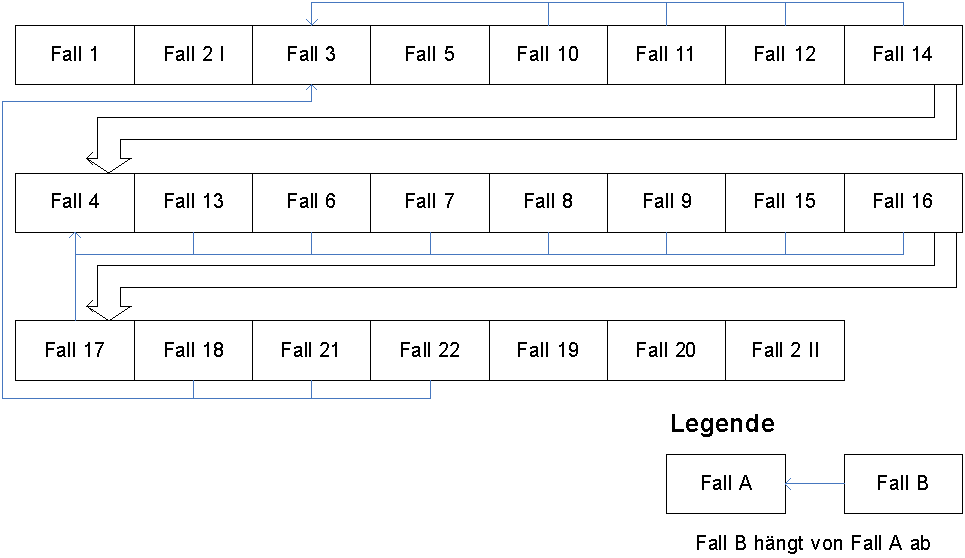
\includegraphics{testplan}

\section{Systemtest}
\begin{longtable}{|c|p{8cm}|c|c|}
\hline
	\textbf{Testfall} & 
	\textbf{Ergebnis} &
	\textbf{korrekt} &
	\textbf{nicht korrekt}\\
\hline\hline
\endhead

 1 & Alle Klassentests geben ``OK'' zurück. & x &  \\\hline
 2 & Speicher wurden angelegt bzw. gelöscht und danach neu angelegt. Neuer Administrator ist angelegt. & x &  \\\hline
 3 & Anzeige aller Ansichten. Kein Speicher wurde geändert. & x &  \\\hline
 4 & Anzeige aller Ansichten, außer gesperrter Ansichten. Kein Speicher wurde geändert. & x &  \\\hline
 5 & Anzeige aller Ansichten, außer gesperrter Ansichten. Kein Speicher wurde geändert. & x &  \\\hline
 6 & Neue Literatur wurde angelegt und wird in Literaturinformation angezeigt. Neue Autoren wurden in Autoren abgelegt und mit Literatur verknüpft. Kein weiterer Speicher wurde geändert. & x &  \\\hline
 7 & Neue Literatur wurde nach Bestätigung angelegt und wird in Literaturinformation angezeigt. Neue Autoren wurden in Autoren abgelegt und mit Literatur verknüpft. Kein weiterer Speicher wurde geändert. & x &  \\\hline
 8 & Literatur wurde geändert und wird in Literaturinformation angezeigt. Neue Autoren wurden in Autoren abgelegt, alte entfernt und neue mit Literatur verknüpft. Kein weiterer Speicher wurde geändert. & x &  \\\hline
 9 & Literatur wurde entfernt. Alte Autoren wurden genauso wie ihre Verknüpfungen entfernt. Kein weiterer Speicher wurde geändert. & x &  \\\hline
10 & Neuer Nutzer wurde angelegt und wird angezeigt. Keine weiteren Speicher wurden geändert. & x &  \\\hline
11 & Fehler wurde beim Anlegen ausgegeben. Keine Speicher wurden geändert. & x &  \\\hline
12 & Nutzer wurde geändert und wird angezeigt. Keine weiteren Speicher wurden geändert. & x &  \\\hline
13 & Eigener Nutzer wurde geändert und wird angezeigt. Keine weiteren Speicher wurden geändert. & x &  \\\hline
14 & Nutzer wurde gelöscht. Keine weiteren Speicher wurden geändert. & x &  \\\hline
15 & Neuer Kommentar wurde angelegt und wird in Literaturinformation angezeigt. Keine weiteren Speicher wurden geändert. & x &  \\\hline
16 & Kommentar wurde geändert und wird in Literaturinformation angezeigt. Keine weiteren Speicher wurden geändert. & x &  \\\hline
17 & Kommentar wurde gelöscht. Keine weiteren Speicher wurden geändert. & x &  \\\hline
18 & Kommentar wurde gelöscht. Keine weiteren Speicher wurden geändert. & x &  \\\hline
19 & Literatur wurde entfernt. Alte Autoren wurden genauso wie ihre Verknüpfungen und Kommentare entfernt. Kein weiterer Speicher wurde geändert. & x &  \\\hline
20 & Nutzer wurde mit dazugehörigen Kommentaren gelöscht. Keine weiteren Speicher wurden geändert. & x &  \\\hline
21 & Alle gesuchten Bücher wurden gefunden, ausgegeben und können ausgewählt werden. & x &  \\\hline
22 & Alle gesuchten Bücher wurden gefunden, ausgegeben und können ausgewählt werden. & x &  \\\hline
\end{longtable}

\section{Abschlußeinschätzung}
Für jede Klasse von Eingaben wurde ein Test durchgeführt. Die Funktionen wurden isoliert als Unittest sowie in realer Umgebung getestet. Die beim abschließenden Systemtest erhaltenen Ergebnisse stimmen mit den erwarteten Ergebnissen überein. Durch dies kann der Systemtest als erfolgreich angesehen werden. Die in der Spezifikation gesetzten Anforderungen wurden erfüllt. Das System kann aus diesem Grund als einsatzbereit angesehen werden. Eine vollkommene Fehlerfreiheit kann trotz der Tests nicht garantiert werden.
